		\ifx \allfiles \undefined		%编译PPT时注释该行
\documentclass{ctexart}				%编译PPT时注释该行
\usepackage{ifthen}
\usepackage[landscape]{geometry}
\usepackage{tikz,units}
\usetikzlibrary{backgrounds,circuits.ee.IEC.relay}

\begin{document}
		\else						%编译PPT时注释该行
			\chapter{吹灰器控制回路}	%编译PPT时注释该行
		\fi						%编译PPT时注释该行
\begin{center}
{\huge 吹灰器控制回路}\\

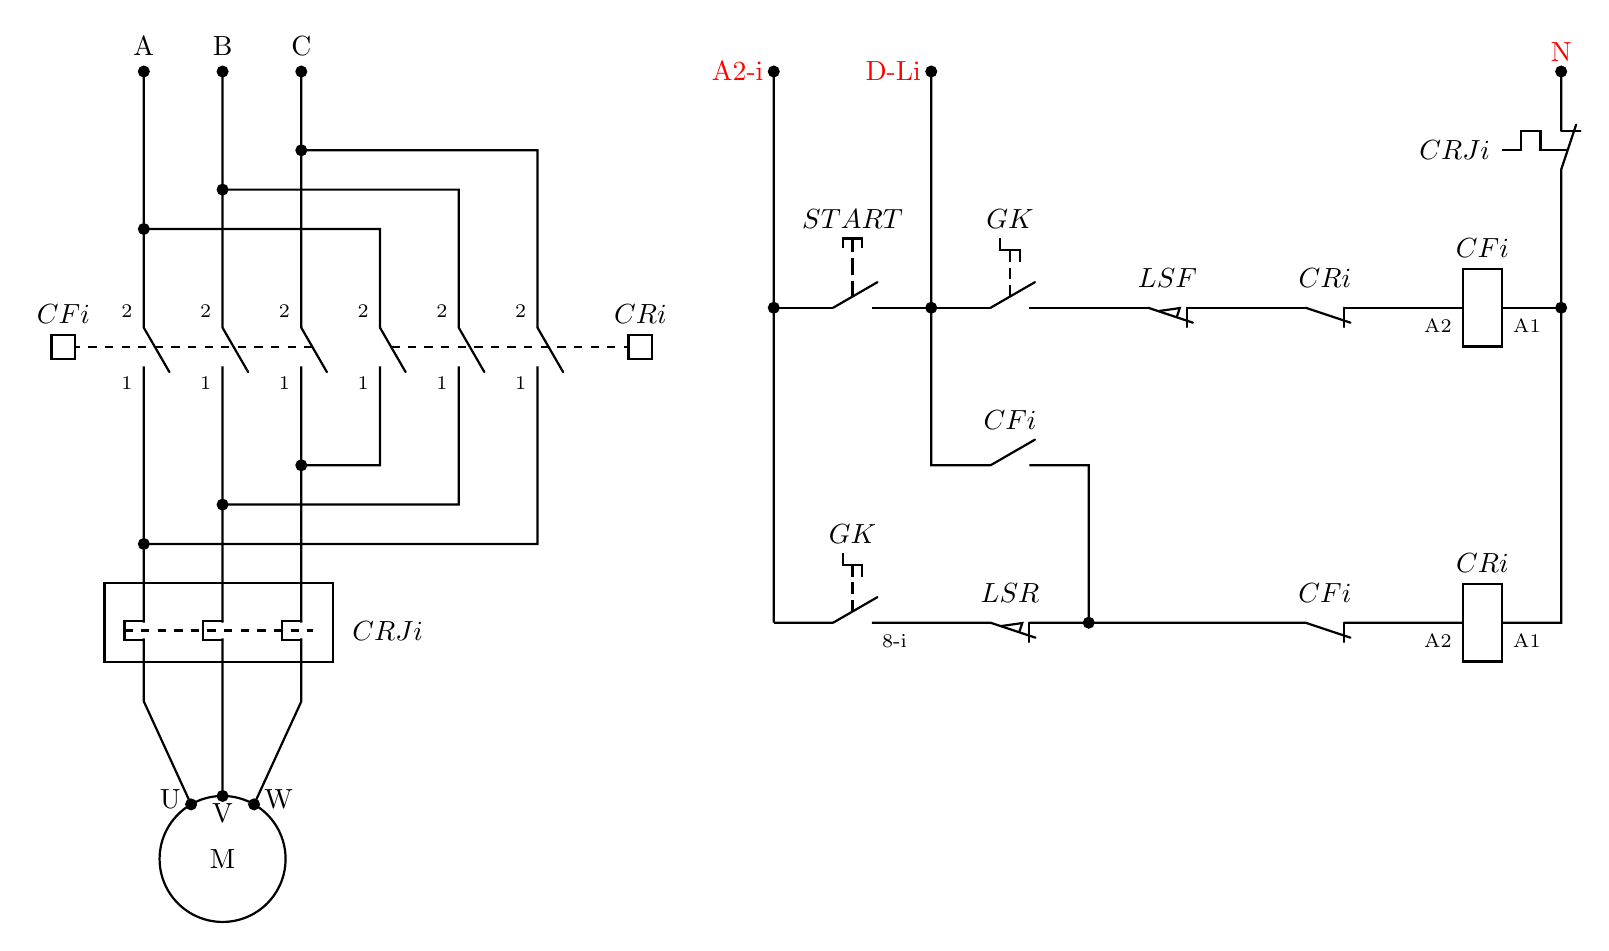
\begin{tikzpicture}[circuit ee IEC relay,thick,scale=2]
		
		

		\draw (4,0)
		to [make contact={turn switch={info=$GK$},term=8-i}] ++(1,0)
		to [break contact={position switch={info=$LSR$}}] ++(1,0)
		node [contact,name=A1]{} -- ++(1,0)
		to [break contact={info=$CFi$}] ++(1,0)
		to [relay coil={info=$CRi$,term=A1,term'=A2}] ++(1,0) -- ++(0,2.5)
		to [break contact={thermal switch={info=$CRJi$}}] ++(0,1)node [contact,name=N]{}
		++(-4,0)node [contact,name=Di]{}
++(-1,0)node [contact,name=L]{} to (4,0);

		\draw (4,2) node[contact]{}
		to [make contact={push button={info=$START$}}] ++(1,0)
		node [contact,name=B1]{}
		to [make contact={turn switch={info=$GK$}}] ++(1,0)
		to [break contact={position switch={info=$LSF$}}] ++(1,0)
		to [break contact={info=$CRi$}] ++(1,0)
		to [relay coil={info=$CFi$,term=A1,term'=A2}] ++(1,0)
		node [contact,name=B2]{};
		
		\draw (Di) -- (B1) -- ++(0,-1) to [make contact={info=$CFi$}] ++(1,0) -- (A1);
		
\node[above,red] at(N) {N};
\node[left,red] at(L) {A2-i};
\node[left,red] at(Di) {D-Li};

\draw (0.5,-1.5) ++(120:0.4)
node [contact,name=U,info={[left]:U}]{};
\draw (0.5,-1.5) ++(90:0.4)
node [contact,name=V,info={[below=1]:V}]{};
\draw (0.5,-1.5) ++(60:0.4)
node [contact,name=W,,info={[right]:W}]{};
\draw (0.5,-1.5) circle (0.4);
\node at(0.5,-1.5) {M};

\draw (0,3.5) node [contact,name=A,info=A]{} -- ++(0,-1)
node [contact,name=A1]{} -- ++(0,-0.5)
to [make contact={term=1,term'=2}] ++(0,-0.5) -- ++(0,-1)
node [contact,name=A2]{}  -- ++(0,-0.5)
to [thermic sensor={name=FR}] ++(0,-0.1) -- ++(0,-0.4)
to (U);

\draw (0.5,3.5) node [contact,name=B,info=B]{} -- ++ (0,-0.75)
node [contact,name=B1]{}  -- ++(0,-0.75)
to [make contact={term=1,term'=2}] ++(0,-0.5) -- ++(0,-0.75)
node [contact,name=B2]{} -- ++(0,-0.75)
to [thermic sensor] ++(0,-0.1) -- ++(0,-0.4)
to (V);

\draw (1,3.5) node [contact,name=C,info=C]{} -- ++ (0,-0.5)
node [contact,name=C1]{}  -- ++(0,-1)
to [make contact={name=KM1,term=1,term'=2}] ++(0,-0.5) -- ++(0,-0.5)
node [contact,name=C2]{} -- ++(0,-1)
to [thermic sensor={info={[right=0.5cm]:$CRJi$}}] ++(0,-0.1) -- ++(0,-0.4)
to (W);
\draw (-0.25,-0.25) rectangle (1.2,0.25);

\draw (A1) -- ++(1.5,0) -- ++(0,-0.5)
to [make contact={name=KM2,term=1,term'=2}] ++(0,-0.5) -- ++(0,-0.5) -- (C2);

\draw (B1) -- ++(1.5,0) -- ++(0,-0.75)
to [make contact={term=1,term'=2}] ++(0,-0.5) -- ++(0,-0.75) -- (B2);

\draw (C1) -- ++(1.5,0) -- ++(0,-1)
to [make contact={term=1,term'=2}] ++(0,-0.5) -- ++(0,-1) -- (A2);

\draw[dashed](KM1.mid) -- ++(-1.5,0)
node[left,draw,solid,minimum size=3mm,label={[above]:$CFi$}]{};

\draw[dashed](KM2.mid) -- ++(1.5,0)
node[right,draw,solid,minimum size=3mm,label={[above]:$CRi$}]{};

\draw[dashed](FR.mid) -- ++(1.2,0);




	\end{tikzpicture}
\\START:就地启动按钮GK:急停旋钮开关D-Li:来至DCS脉冲指令接通后过来的220VAC电压\\
LSF:退到位限位开关LSR:进到位限位开关CFi:前进交流接触器CRi:后退交流接触器CRJi:热继电器
\end{center}
		\ifx \allfiles \undefined
\end{document}

\fi
